\documentclass[12pt]{article}
\usepackage{amsmath}
\usepackage{amsfonts}
\usepackage{amssymb}
\usepackage[utf8]{inputenc}
\usepackage[T1,T2A]{fontenc}
\usepackage[english, russian]{babel}
\usepackage{graphicx}
\usepackage{float}
\usepackage[left=2cm,right=2cm,top=2cm,bottom=2cm]{geometry}
\usepackage{wrapfig}
\usepackage{pgfplots}
\usepackage{setspace}
\usepackage{indentfirst}
\usepackage{subfigure}
\usepackage{hyperref}
\usepackage{mathrsfs}

\hypersetup{
    colorlinks=true,
    linkcolor=red,
    urlcolor=magenta,
}

\graphicspath{{pictures}}

\title{
    Лабораторная работа 2.4.1 \\
    <<Определение теплоты испарения жидкости>>
}

\author{Балдин Виктор, Б01-303}

\begin{document}
    \maketitle
    \paragraph{Цель работы}
    \begin{enumerate}
        \item Измерение давления насыщенного пара жидкости при различной
        температуре.
        \item Вычисление теплоты испарения с помощью уравнения Клайперона-
        Клаузиуса.
    \end{enumerate}
    \paragraph{Оборудование} Термостат, герметичный сосуд, заполненный
    исследуемой жидкостью, отсчетный микроскоп.

    \section{Теоретическая часть}
    Для теплоты испарения можно записать уравнение Клайперона-Клаузиуса:
    \begin{equation}
        \frac{dP}{dT} = \frac{L}{T(V_2 - V_1)},
        \label{klaus}
    \end{equation}
    где $V_2$ -- объем газа, $V_1$ -- объем жидкости.

    В данном случае мы используем модель идеального газа применительно
    к парам исследуемой жидкости:
    \begin{equation}
        V = \frac{RT}{P}
        \label{klaip}
    \end{equation}

    Объединяя \ref{klaus} и \ref{klaip}, получим:
    \begin{equation}
        L = \frac{RT^2}{P}\frac{dP}{dT} = -R\frac{d(\ln P)}{d(1 / T)}
        \label{L}
    \end{equation}

    Или в интегральной форме:
    \begin{equation}
        P = P_0 \exp \left(\frac{L}{R}\left(\frac{1}{T_0} - \frac{1}{T}\right)\right)
        \label{integral}
    \end{equation}

    \section{Установка}
    Схема экспериментальной установки приведена на рисунке \ref{stand}.
    Погрешности: термостат -- 0.1 \textdegree C, манометр -- 0.1 мм. рт. ст..

    \begin{figure}[h!]
        \centering
        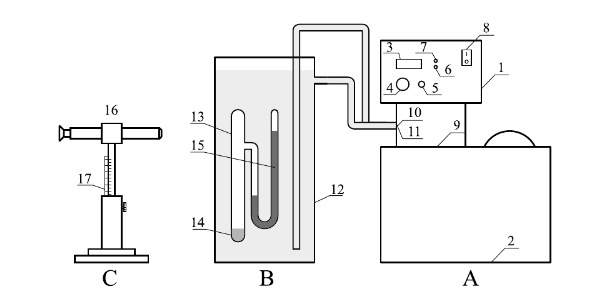
\includegraphics[scale=1]{stand.png}
        \caption{Схема установки для определения удельной теплоты испарения}
        \label{stand}
    \end{figure}

    \section{Ход работы}
    \begin{enumerate}
        \item Измерим разность уровней в ртутном U-образом манометре с помощью
        микроскопа.
        \item Включим термостат.
        \item Будем измерять давление насыщенного пара с интервалом 1 \textdegree C
        до 40 \textdegree C.
        Данные занесем в таблицу \ref{heat}.
        \item Теперь установим термостат на комнатную температуру и снимем еще немного
        точек при охлаждении с интервалом 2 \textdegree C для верификации результатов
        предыдущего пункта. Результаты в таблице \ref{cool}. Систематические погрешности
        для величин $1/T$ и $\ln P$ много меньше случайных.

        \begin{table}[H]
            \centering
            \begin{tabular}{|c|c|c|c|}
            \hline
            $T$, \textdegree C  & $P$, мм. рт. ст.      & $1/T$, K$^{-1}$  & $\ln P$  \\ \hline
            23 & 47.70  & 3.38 & 3.86 \\ \hline
            24 & 49.96  & 3.37 & 3.91 \\ \hline
            25 & 52.05  & 3.36 & 3.95 \\ \hline
            26 & 54.19  & 3.34 & 3.99 \\ \hline
            27 & 58.38  & 3.33 & 4.07 \\ \hline
            28 & 61.95  & 3.32 & 4.13 \\ \hline
            29 & 66.56  & 3.31 & 4.20 \\ \hline
            30 & 70.81  & 3.30 & 4.26 \\ \hline
            31 & 74.65  & 3.29 & 4.31 \\ \hline
            32 & 79.05  & 3.28 & 4.37 \\ \hline
            33 & 84.40  & 3.27 & 4.44 \\ \hline
            34 & 89.56  & 3.26 & 4.49 \\ \hline
            35 & 93.99  & 3.25 & 4.54 \\ \hline
            36 & 97.62  & 3.24 & 4.58 \\ \hline
            37 & 104.13 & 3.23 & 4.65 \\ \hline
            38 & 110.42 & 3.22 & 4.70 \\ \hline
            39 & 116.00 & 3.21 & 4.75 \\ \hline
            40 & 121.86 & 3.19 & 4.80 \\ \hline
            \end{tabular}
            \caption{Измерения $P(T)$ при нагревании}
            \label{heat}
        \end{table}

        \begin{table}[H]
            \centering
            \begin{tabular}{|c|c|c|c|}
            \hline
            $T$, \textdegree C  & $P$, мм. рт. ст.      & $1/T$, K$^{-1}$  & $\ln P$  \\ \hline
            40 & 121.86 & 3.19 & 4.80 \\ \hline
            38 & 108.81 & 3.22 & 4.69 \\ \hline
            36 & 99.01  & 3.24 & 4.60 \\ \hline
            34 & 89.86  & 3.26 & 4.50 \\ \hline
            \end{tabular}
            \caption{Измерения $P(T)$ при охлаждении}
            \label{cool}
            \end{table}

        \item Построим графики по полученным данным в координатах
        $P(T)$ на рис. \ref{curve} и $\ln P(1/T)$ на рис. \ref{lin}.
        Для графика $P(T)$ проведем наилучшую кривую, соответветствующую формуле
        \ref{integral}, пользуясь методом МНК.

        \begin{figure}[H]
            \centering
            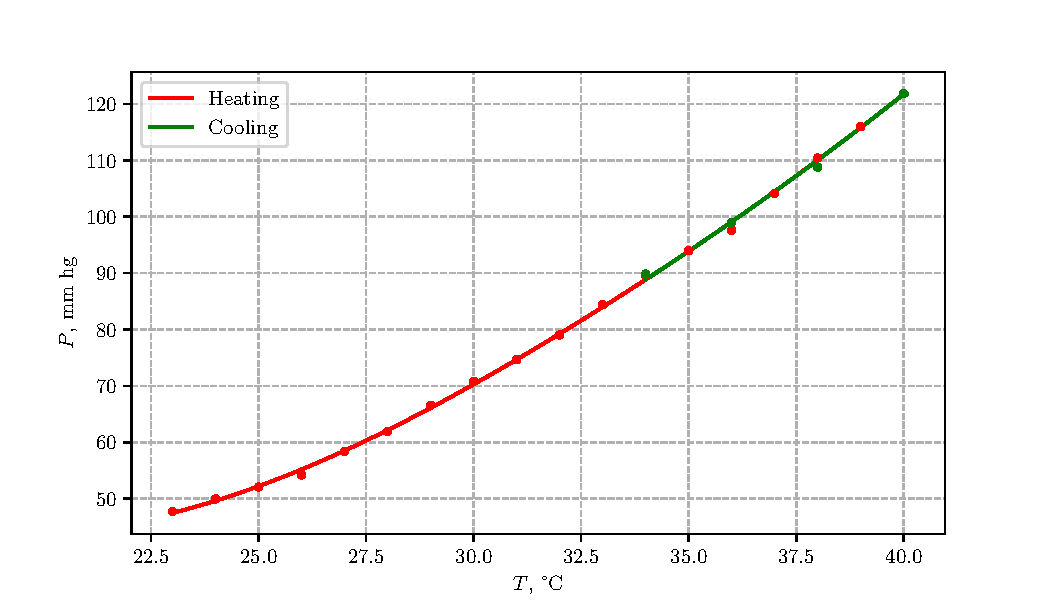
\includegraphics{data/curve.pdf}
            \caption{Зависимость $P(T)$}
            \label{curve}
        \end{figure}

        \begin{figure}[H]
            \centering
            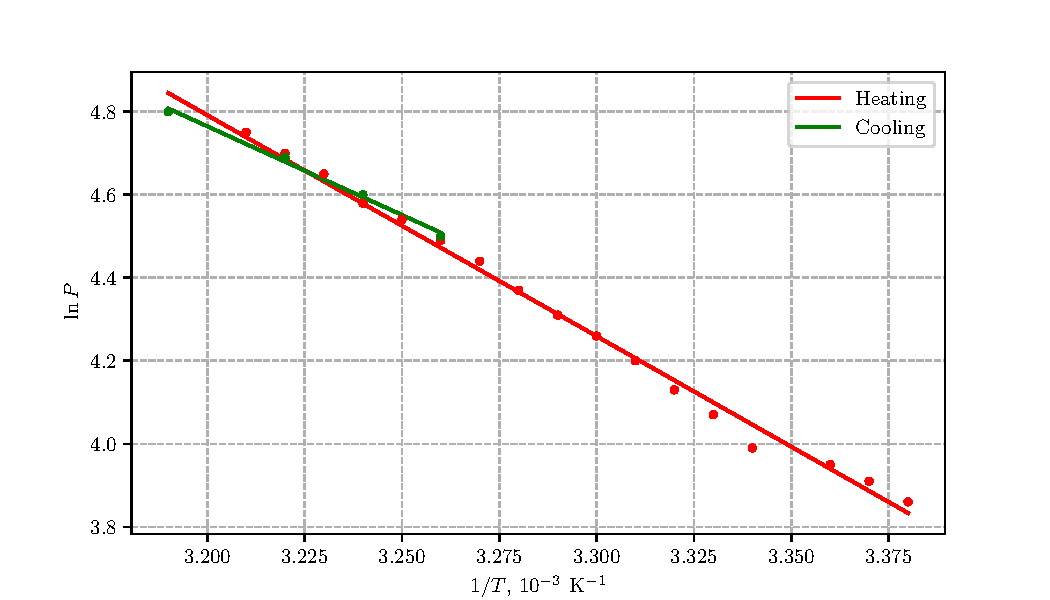
\includegraphics{data/lin.pdf}
            \caption{Линеаризованная зависимость $\ln P(1 / T)$}
            \label{lin}
        \end{figure}

        \item По линеаризованному графику:
        $$
        \frac{d(\ln P)}{d(1/T)} = (-5.3 \pm 0.1)\cdot 10^3\ \text{K}, \ \varepsilon = 2\%
        $$
        При этом погрешность считалась равной случайной погрешности аппроксимации, в силу
        малости приборных: $\sigma \approx \sigma^{\text{случ}}$.
        Отсюда по формуле \ref{L} получим:
        $$
        L = (44.0 \pm 0.9)\ \text{кДж} / \text{моль},\ \varepsilon = 2\%
        $$

        \item Получим $L$ из изначального графика. Для этого проведем касательные к графику
        в начале, в середине и в конце (см. рис. \ref{curve}). Из аппроксимации получим:
        $$
        L = (43.6\pm 0.9)\ \text{кДж} / \text{моль},\ \varepsilon = 2\%
        $$
        Усреднив полученные значения, найдем:
        $$
        \overline{L} = (43.8 \pm 0.9)\ \text{кДж}/\text{моль},\ \varepsilon = 2\%
        $$
    \end{enumerate}

    \section{Вывод}
    Полученные нами разными методами значения теплты испарения $L$ лежат
    в пределах погрешности друг друга. Табличное значение для нормальных
    условий $L_{\text{табл}} = 40.7$ кДж/моль. Это не слишком отличается
    от измеренного нами. Значит, эксперимент можно считать довольно
    качественным.
\end{document}
